\documentclass{beamer}
\usetheme{Singapore}
\setbeamercovered{transparent}

\usepackage{ dsfont }
\usepackage{ amsmath }
\usepackage{ mathrsfs }
\usepackage{ amssymb }
\usepackage{ amsthm }
\usepackage{ graphicx }
 
\usepackage[utf8]{inputenc}

\newcommand{\Prob}{\mathbb{P}}

\AtBeginSection[]
{
	\begin{frame}
		\frametitle{Table of Contents}
		\tableofcontents[currentsection]
	\end{frame}
} 
 
 
%Information to be included in the title page:
\title{Statistical Models for Bursty Events}
%\subtitle{}
\author{Smarak Nayak}
\date{October 4, 2016}
 
 
\begin{document}
 
\frame{\titlepage}
\section{Introduction}

\begin{frame}{Motivation}
	Classical extreme value theory assumes that events happen uniformly. \\~\\
	
	However this is not always the case, in many systems the events occur in bursts. \\~\\
	
	Examples include both human-created events and physical phenomena:
		\begin{itemize}
		\item Communication
		\item Financial Trades 
		\item Network Traffic
		\item Neuron Firing Sequences
		\item Seismic Activity
	    \end{itemize}
	
\end{frame}

\begin{frame}{Example Process }
    \begin{figure}
        %\centering
        \hspace{-0.5cm}
        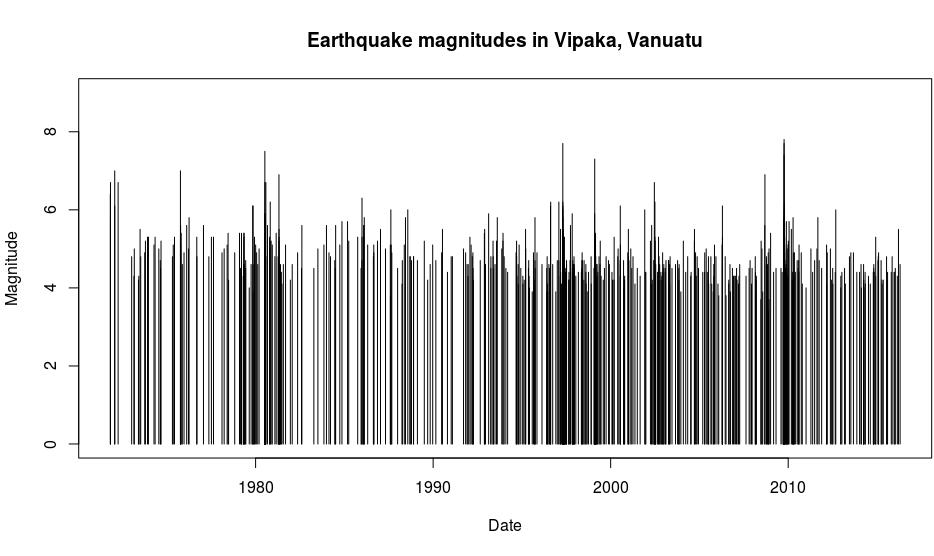
\includegraphics[scale=0.45]{EarthQuakeData.jpeg}
        %\caption{Caption}
        %\label{fig:my_label}
    \end{figure}

\end{frame}

\begin{frame}{Example Process After Thresholding}
    \begin{figure}
        %\centering
        \hspace{-0.8cm}
        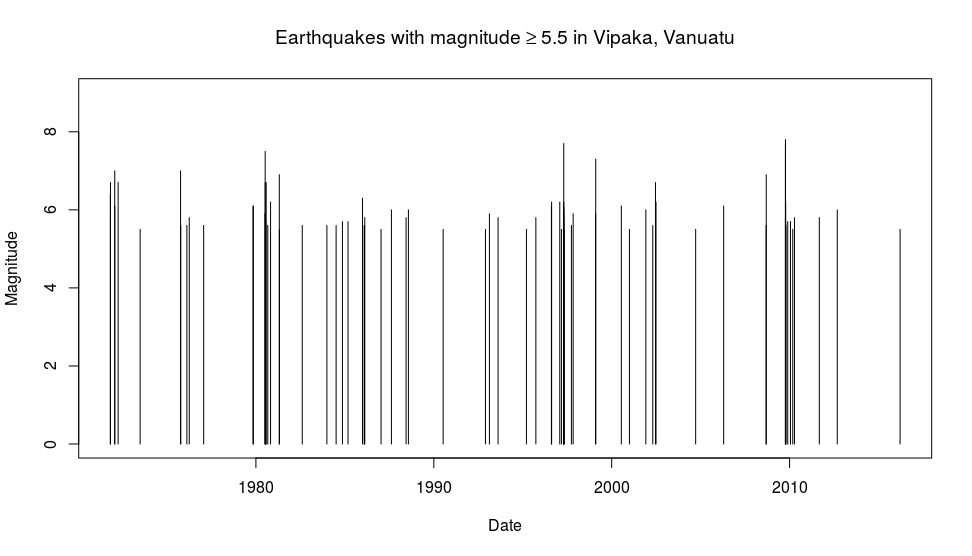
\includegraphics[scale=0.45]{ThresholdedEQData.jpeg}
        %\caption{Caption}
        %\label{fig:my_label}
    \end{figure}
\end{frame}
 
\begin{frame}{Notation}
	
	Let $J_1 , J_2 , ...$ be a sequence of i.i.d. random variables that model the jump sizes (event magnitudes).
	\\~\\
	Let $W_1, W_2, ...$ be a sequence of i.i.d positive random variables that model the waiting times between the jumps.
	\\~\\
	We can then define $(W_1 , J_1 ), (W_2 , J_2 ), ...$ to be a sequence of i.i.d $\mathbb{R} \times \mathbb{R} ^+$ random variables.
\end{frame}

\begin{frame}{Notation Contd.}
    Now define the sum of the first $n$ waiting times to be $S(n):=\sum^n_{i=1} W_i$
    \\~\\
    Define a renewal process $N(t):=\max\{n\geq0:S(n)\leq t\}$
    \\~\\
    Finally we define the Continuous Time Random Maxima (CTRM) to be $M(t) := \bigvee_{k=1}^{N(t)} J_k
= \max\{J_k: k = 1, \ldots, N(t)\}, \quad t \ge 0.$
\end{frame}

\begin{frame}{CTRM Example}
    \begin{figure}
        \centering
        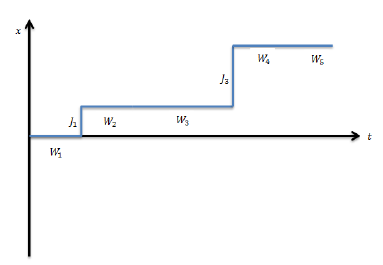
\includegraphics[scale=1]{CTRM.png}
        %\caption{Caption}
        %\label{fig:my_label}
    \end{figure}
\end{frame}

\begin{frame}{ A Possible Simulation }
	We assume that the waiting times and jump sizes are independent.
	\\~\\
	Waiting times $W_i$ are simulated according to a stable distribution with stability parameter $\beta \in (0,1)$, skewness parameter 1, location parameter 0, and scale parameter =1.
	\\~\\
	Jump sizes $J_i$ are simulated according to Generalized Extreme Value (GEV) distribution with location parameter $\mu$, scale parameter $\sigma$ and shape parameter $\xi$.
	\\~\\
	The primary goal is to design methodology that fits models to the CTRM of the simulated data.
\end{frame}

\begin{frame}{Simulated data}
    \begin{center}
        $\beta=0.7, \mu=0, \sigma=1, \xi=0.3$
    \end{center}
	\begin{figure}
        \centering
        \vspace{-0.5cm}
        \hspace{-0.8cm}
        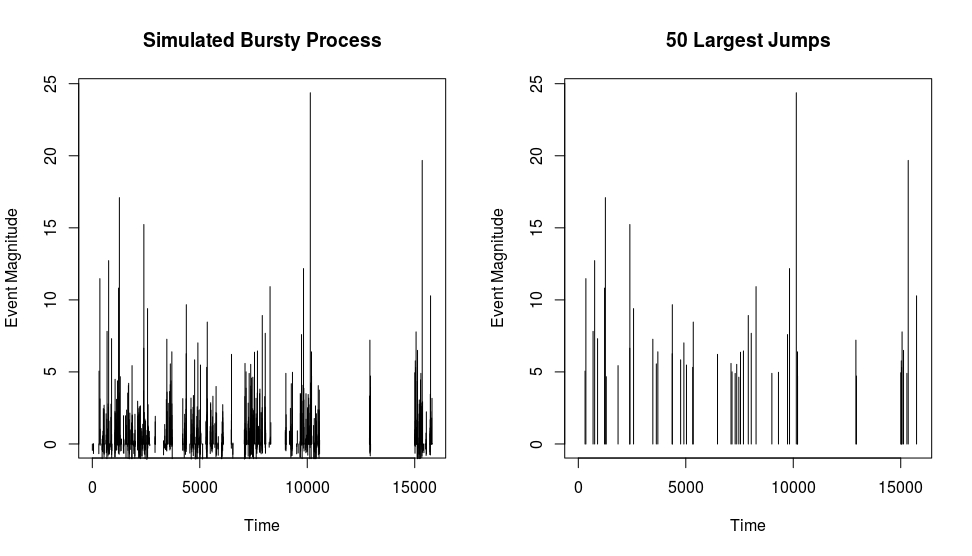
\includegraphics[scale=0.45]{SimulatedBursty.jpeg}
        %\caption{Caption}
        %\label{fig:my_label}
    \end{figure}
\end{frame}

\section{Limit theorems}

\begin{frame}{Scaling Limit of Waiting Times}
	Since we will be working with limits, we need to define partial processes.
	\\~\\
	Define the partial sum-process as $S_p(t):=\sum^{\lfloor{t}\rfloor}_{i=1} W_i$
	\\~\\
	\begin{block}{Theorem (Meerschaert and Sikorskii (2011))}
		Suppose that $W_i$ are i.i.d. and positive with $\Prob(W_n>t)=ct^{-\beta}$ for all $t>c^{1/\beta}$, some $c>0$ and $0<\beta<1$, then
		\[
		    \{b(c)^{-1}S_p(ct)\}_{t\geq0} \xrightarrow[c\to \infty]{J_1} \{D(t)\}_{t\geq0},
		\]
		where $\{D(t)\}_{t\geq0}$ is $\beta$-stable subordinator and $b(c)=c^{1/\beta}.$
	\end{block}
\end{frame}



\begin{frame}{Scaling Limit of Maxima}
	\begin{block}{Theorem (Lamperti (1964))}
		Let $F(x)$ be the CDF of $J_i$. Now suppose there exists constants $a(n)>0$ and $d(n)$ such that,
		\[
		    \Prob\left(\bigvee_{i=1}^n J_i\leq a(n)^{-1}(x-d(n))\right)=F^n(a(n)^{-1}(x-d(n))) \xrightarrow[n\to \infty]{d} G(x).
		\]
		Then $G(x)$ must be a member of the GEV family. Now define the partial max-process as
		\[
	        M_p(t):=
	        \begin{cases}
	            \bigvee_{i=1}^{\lfloor{t}\rfloor} J_i, &\textrm{$t\geq 1$}\\
	            J_1, &\textrm{$0<t<1.$}
	        \end{cases}
		\]
		Then $\{a(c)^{-1}(M_p(ct)-d(c))\}_{t\geq0} \xrightarrow[c\to \infty]{J_1} \{A(t)\}_{t\geq0}$, where $\{A(t)\}_{t\geq0}$ is an extremal process generated by G.
	\end{block}
\end{frame}

\begin{frame}{Scaling Limit of the Joint Process}
    \begin{block}{Theorem}
        Let $(W_i,J_i)$ be a sequence of i.i.d $\mathbb{R}^+\times\mathbb{R}$ random vectors such that
        \[
            \{b(c)^{-1}S_p(ct),a(c)^{-1}(M_p(ct)-d(c))\}_{t\geq0} \xrightarrow[c\to \infty]{J_1} \{(D(t),A(t))\}_{t\geq0}
        \]
        where the paths of $\{D(t))\}_{t\geq0}$ are non-decreasing almost surely. Then,
        \[
            \{a(n)^{-1}(M(ct)-d(n))\}_{t\geq0} \xrightarrow[c\to \infty]{J_1} \{(A(E(t))\}_{t\geq0},
        \]
        where $E:=\inf \{u>0:D(u)>t\}$ is the inverse of $D$ and $n= \tilde{b}(c)$ where $\tilde{b}(c)$ is the asymptotic inverse of $b(c)$.
    \end{block}
\end{frame}

\section{Distribution of the CTRM}

\begin{frame}{Variables of Interest}

    \begin{figure}
        \centering
        \vspace{-0.5cm}
        \hspace{-0cm}
        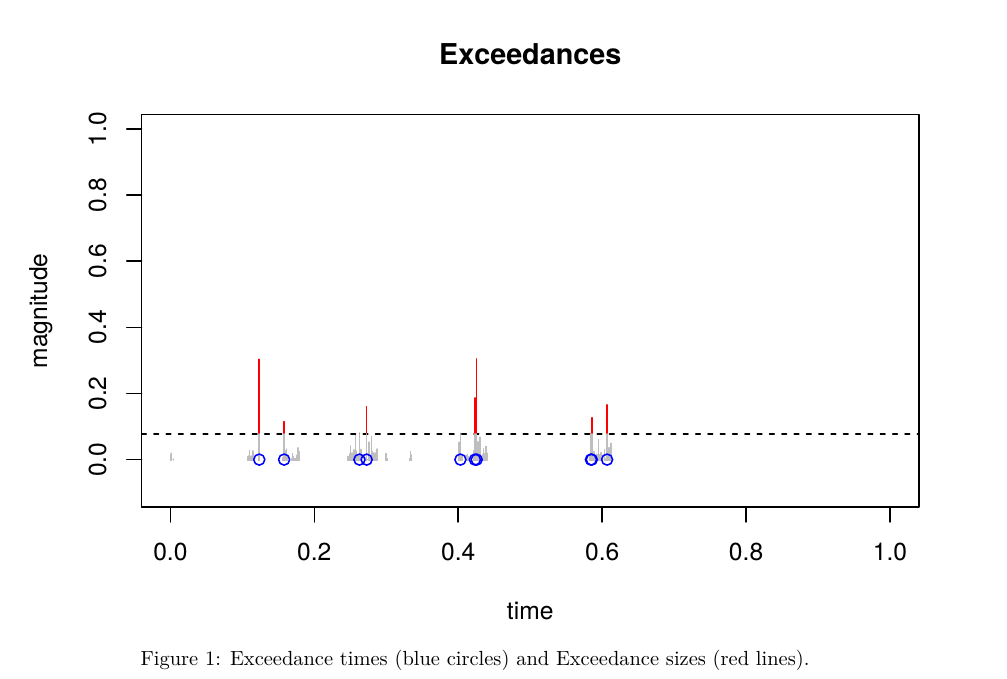
\includegraphics[scale=0.3]{Exceedances.png}
        %\caption{Caption}
        %\label{fig:my_label}
    \end{figure}
    We are interested in modelling the durations $T_\ell := \inf\{t: M(t) > \ell\}$ and the exceedances $X_\ell=M(T_\ell)-\ell$    
\end{frame}



\begin{frame}{Distribution of Durations}
    \begin{block}{Proposition (Meerschaert and Stoev (2007))}
         Let $\ell$ be the threshold level, then define $\xi_\ell := \inf\{t: A(E(t)) > \ell\}$ as the hitting time of level
	$\ell$ by the process $A(E(t))$. Then
        \[
            \xi_\ell \sim (-\log F(\ell))^{\frac{-1}{\beta}}V_{\beta,1}.
        \]
        Where F is the cdf of a GEV random variable and $V_{\beta,1}$ is a Mittag-Leffler RV with tail parameter $\beta$ and scale parameter $1$.
        \end{block}
        Using this result it can be shown that 
        \[
            T_\ell \sim ML(\beta,\delta),
        \]
        with $\delta=b(n)(-\log F(\ell))^{-1/\beta}$.

    
\end{frame}

\begin{frame}{Distribution of Exceedances}
    \begin{block}{Theorem (Coles (2001))}
         If $J_1,J_2,\ldots$ are a sequence of i.i.d. random variables such that
        \[
            \Prob(\max(J_1,\ldots,J_n)\leq z)\xrightarrow[n\to\infty]{}G(z).
        \]
        Where G is the cdf of a GEV$(\xi,\mu.\sigma)$ random variable, then we have
        \[
            X_\ell \sim GP(\xi,\tilde{\sigma}),
        \]
        with $\tilde{\sigma}=\sigma+\xi(\ell-\mu)$.
    \end{block}
\end{frame}

\section{Parameter Estimation of Simulated Data}

\begin{frame}{Stability Plots}
    \begin{figure}
        \centering
        \vspace{-0.5cm}
        \hspace{-0cm}
        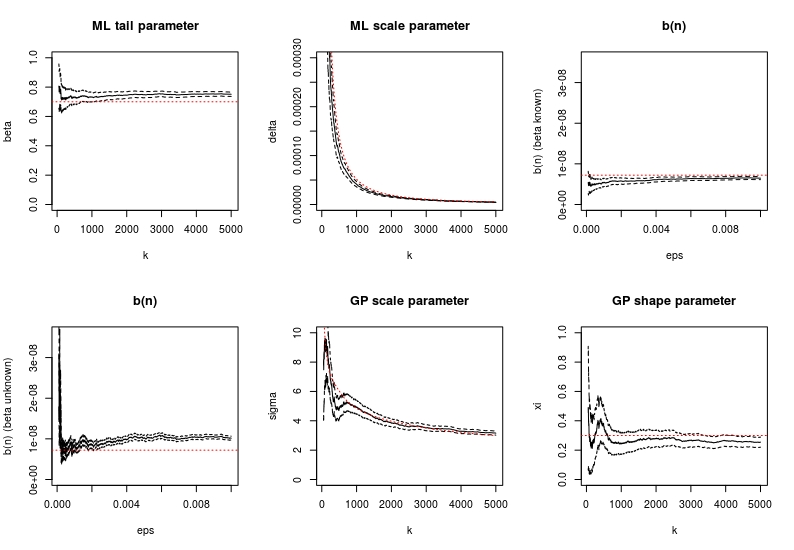
\includegraphics[scale=0.45]{ParameterThresholdPlots.jpeg}
        %\caption{Caption}
        %\label{fig:my_label}
    \end{figure}
\end{frame}

\begin{frame}{Threshold Selection}
If the model fits the data well we should have $\beta, b(n), \xi$ constant and $\sigma$ linear with respect to the threshold level $\ell$.
\\~\\
At high thresholds we have a small amount of data points and thus a high variance.
\\~\\
Since exceedances and durations are GP and ML distributed asymptotically low thresholds introduce bias.
\\~\\
When picking a threshold we should attempt to minimise the variance whilst keeping the threshold high.
\end{frame}

\begin{frame}{Further Research}
Apply the model to datasets with heavy tail waiting times such as bond futures trades, seismic activity and network transmissions.
\\~\\
Extend the model to include the case where there is a dependence structure between $W_i$ and $J_i$.
\end{frame}
 
\end{document}